\chapter{Gaussian Mixture Models}
\label{ch:gmm}

\section{Motivation: Clustering}

Suppose you are given the set of points in the left hand side of Figure~\ref{fig:clustering-example}, and you are asked to devise an algorithm to automatically find $K$ clusters. One option is the following:
\begin{enumerate}
    \item Initialise randomly $K$ centroids.
    \item Assign each data point to the closes centroid.
    \item Recompute centroids from the assignments.
    \item Iterate the past two steps.
\end{enumerate}\vspace{3mm}

This is called the $K$-means algorithm, and it results on the color-coded assignment shown in the center of Figure~\ref{fig:clustering-example}.

\begin{figure}[H]
    \centering
    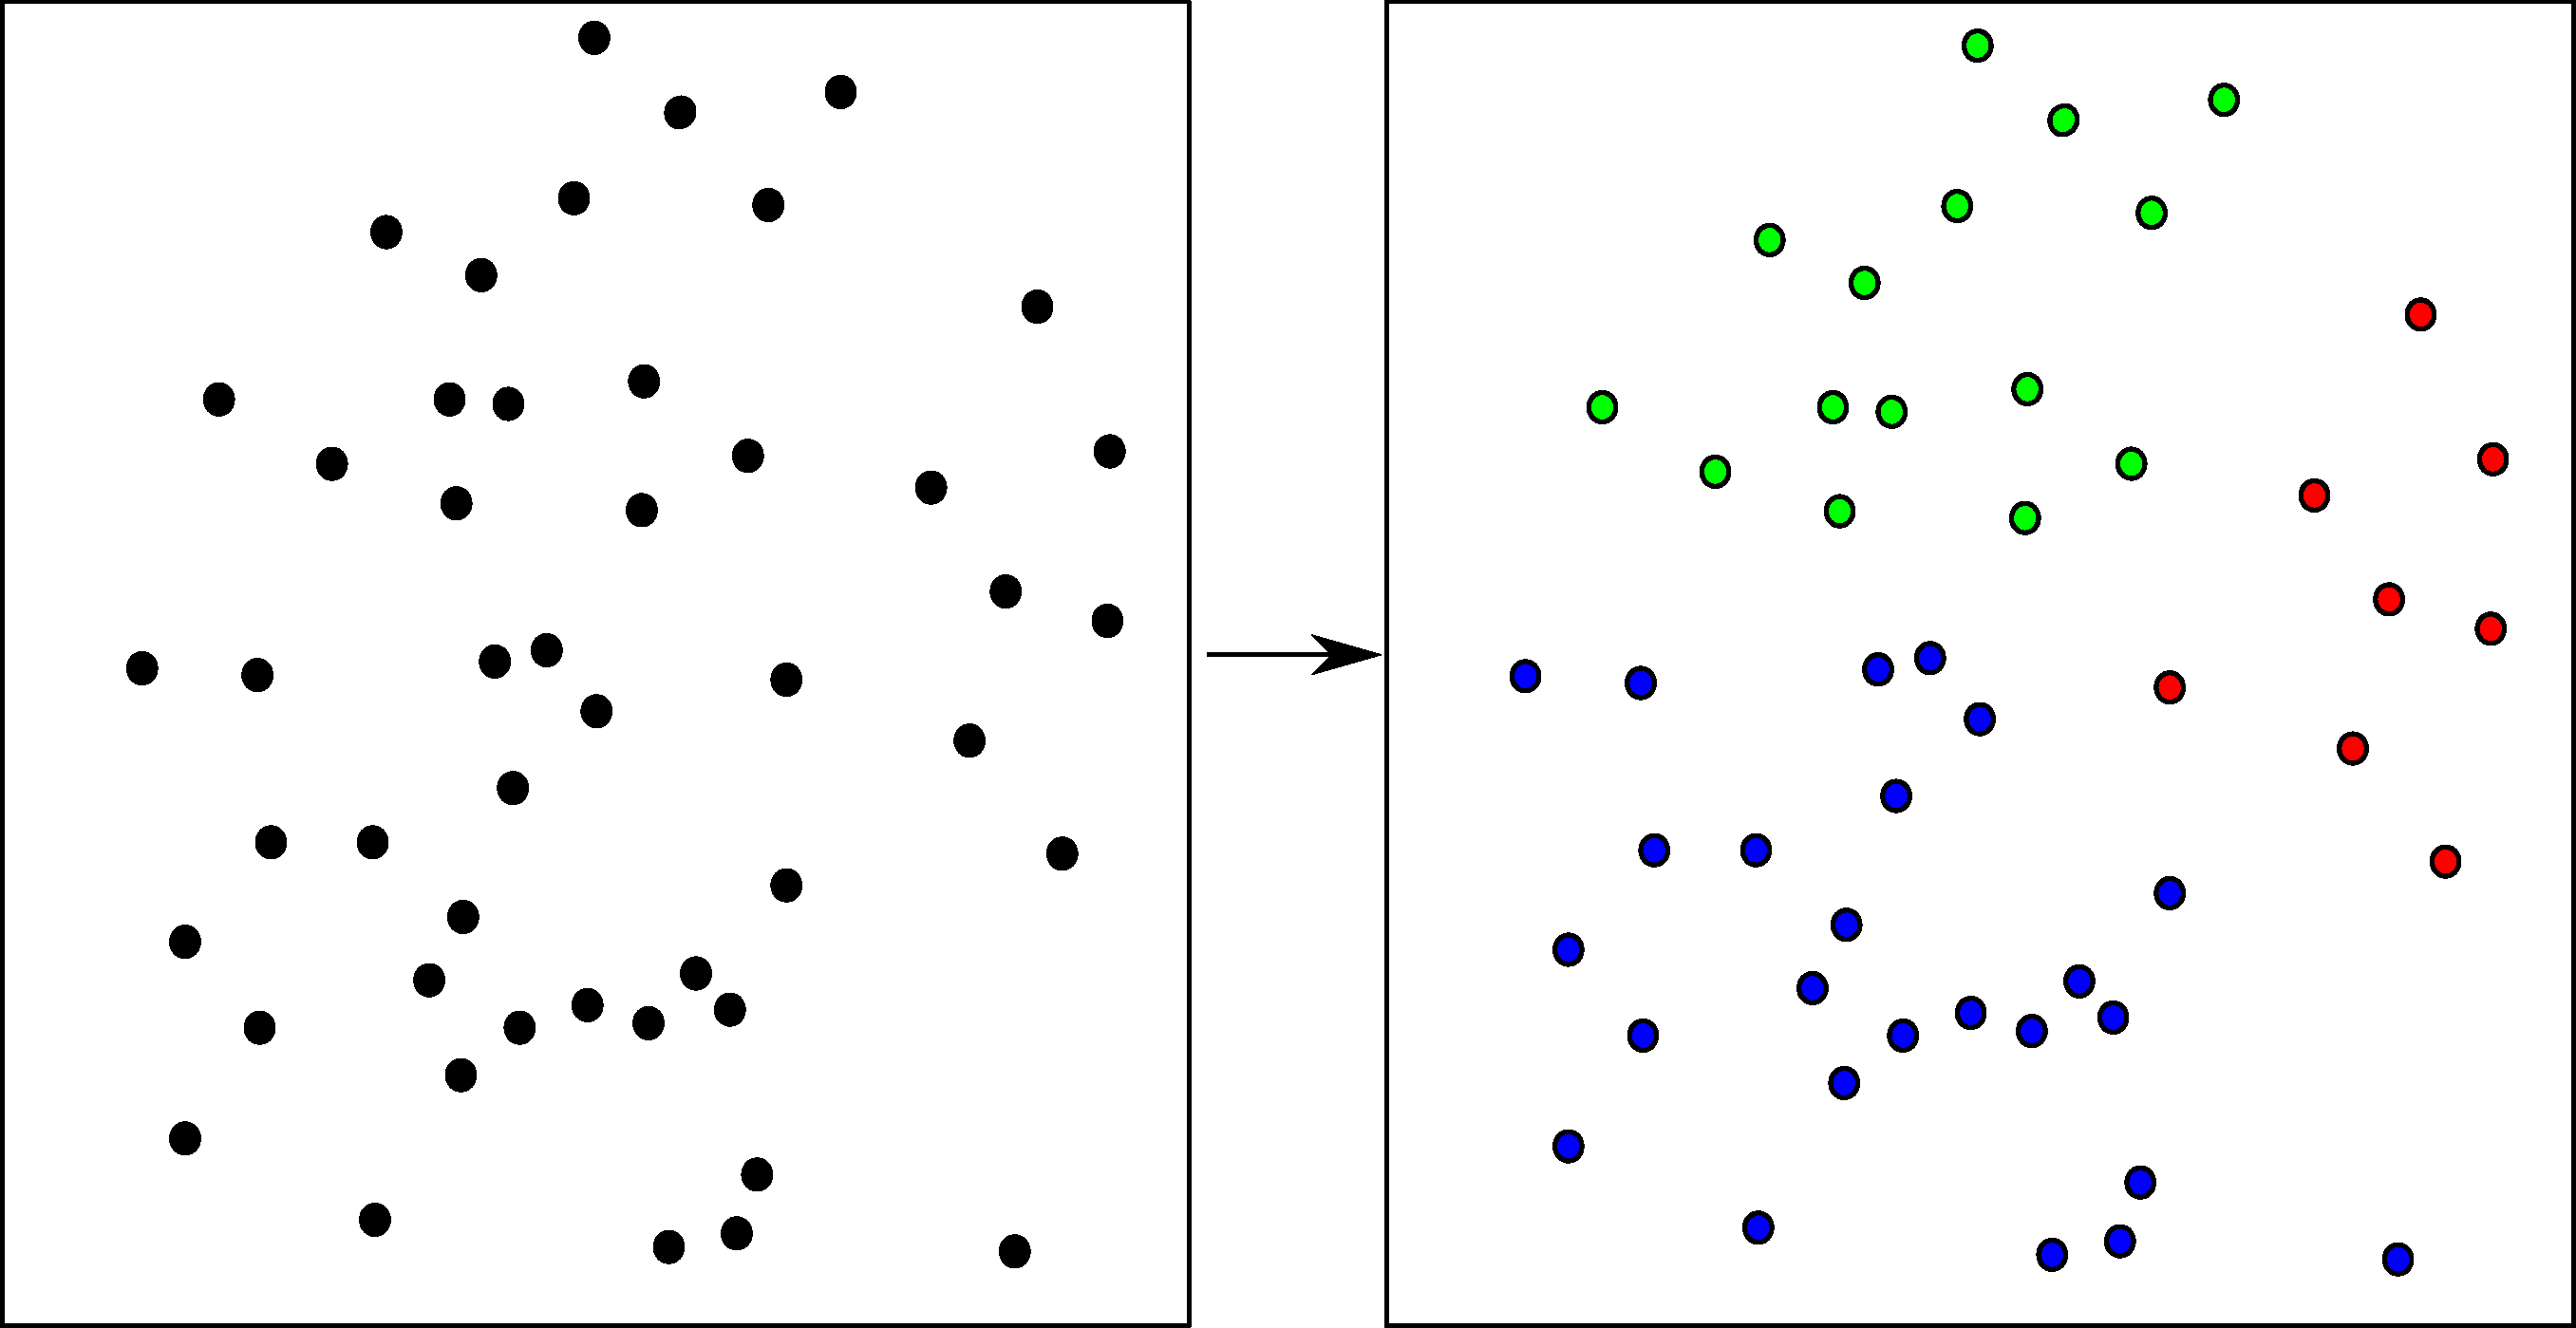
\includegraphics[width=0.3\textwidth]{fig/clustering}
    \hfill
    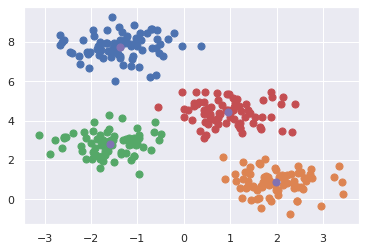
\includegraphics[width=0.3\textwidth]{fig/clustering_done}
    \hfill
    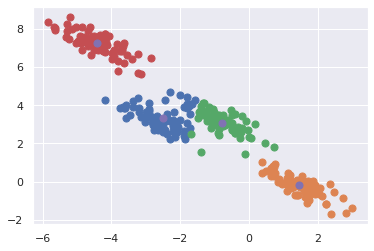
\includegraphics[width=0.3\textwidth]{fig/clustering_fail}
    \caption{Clustering example.\label{fig:clustering-example}}
\end{figure}

Important properties of the $K$-means algorithm:
\begin{itemize}
 \item Automatic inference of latent variables. The point-to-cluster assignment variable is \textbf{unknown}/\textbf{latent}/\textbf{hidden}, and must be infered together with the parameters.
 \item Limited to spherical and equally populated clusters. Because the assignment criterion is the Euclidean distances, see the right hand side of Figure~\ref{fig:clustering-example}.
\end{itemize}


\remark{gmm-def}{Gaussian mixture model (GMM):
\begin{itemize}
 \item For each data point $\bs{x}_n$ there is a hidden variable $z_n$ taking discrete values from 1 to $K$: $z_n\in\{1,\ldots,K\}$.
 \item Its prior probability is defined as: $p(z_n=k)=\pi_k$, $\sum_{k=1}^K \pi_k = 1$.
 \item Given $z_n$, the data point is modeled as a multivariate Gaussian:
 \begin{equation}
   p(\bs{x}_n|z_n=k) = \mathcal{N}(\bs{x}_n;\bs{\mu}_k,\bs{\Sigma}_k)
 \end{equation}
\end{itemize}
}

Advantages:
\begin{enumerate}
\item Having $\pi_1,\ldots,\pi_K$ means that groups can be differently populated.
\item The shape of the groups is modeled by $\bs{\Sigma}_k$.
\end{enumerate}

\section{Maximum Likelihood for GMM: the Expectation-Maximisation algorithm}
 Let's compute $p(\bs{x}_n)$:
 \begin{equation} p(\bs{x}_n) = \sum_{k=1}^K p(\bs{x}_n,z_n=k) = \sum_{k=1}^K \pi_k\mathcal{N}(\bs{x}_n;\bs{\mu}_k,\bs{\Sigma}_k).\end{equation}
 The log-likelihood writes:
 \begin{equation}\mathcal{L}(\bs{\Theta}|\bs{X}) = \sum_{n=1}^N \log  \sum_{k=1}^K \pi_k\mathcal{N}(\bs{x}_n;\bs{\mu}_k,\bs{\Sigma}_k),\end{equation}
 with $\bs{\Theta}=\{\pi_k,\bs{\mu}_k,\bs{\Sigma}_k\}_{k=1}^K$. One can easily check by computing $\displaystyle\frac{\partial\mathcal{L}}{\partial\pi_k}$, $\displaystyle\frac{\partial\mathcal{L}}{\partial\bs{\mu}_k}$ or $\displaystyle\frac{\partial\mathcal{L}}{\partial\bs{\Sigma}_k}$ that direct optimisation is very complicated.\vspace{3mm}

Notice that $\log p(\mathbf{x})$ is not a nice function to take the derivative of, but that $\log p(\bs{x},z)$ is. However, $z$ is not observed and we need to take some sort of expectation. We will do that w.r.t.\ the posterior distribution, and this choice will be justified later on.\vspace{2mm}\\
\remark{ecdll-def}{The expected complete-data log-likelihood writes:
 \begin{equation}\mathcal{Q}(\bs{\Theta},\bs{\Theta}^0) = \mathbb{E}_{p(z|\bs{x};\bs{\Theta}^0)} \log p(\bs{x},z;\bs{\Theta})\end{equation}
}\vspace{3mm}

\remark{em-gmm}{We can now propose the EM algorithnm for GMM, with some notation first: observations $\bs{X}=\{\bs{x}_n\}_{n=1}^N$, latent variables $\bs{Z}=\{z_n\}_{n=1}^N$ and parameters $\bs{\Theta}=\{\pi_k,\bs{\mu}_k,\bs{\Sigma}_k\}_{k=1}^K$. Given $\bs{\Theta}^0$, we use the expected complete-data log-likelihood $\mathcal{Q}$:\vspace{2mm}
\begin{enumerate}
  \item Expectation: 
  \begin{equation} \mathcal{Q}(\bs{\Theta},\bs{\Theta}^0) = \mathbb{E}_{p(\bs{Z}|\bs{X};\bs{\Theta}^0)} \log p(\bs{Z},\bs{X};\bs{\Theta})
  \end{equation}
  \item Maximisation: 
  \begin{equation} \bs{\Theta}^1 = \arg\max_{\bs{\Theta}} \mathcal{Q}(\bs{\Theta},\bs{\Theta}^0)\end{equation}
\end{enumerate}
}

  We can look back to $K$-means:
 \begin{enumerate}
  \item Infer latent variables (assignment) given the parameters (centroids).
  \item Estimate the parameters (centroids) given the assignments.
 \end{enumerate} 

\begin{tabular}{lll}
 \toprule
  Algorithm & $K$-means & EM for GMM \\
  \midrule
  Criterion & Sum Euclidean distance to assigned cluster center & Expected complete-data log-likelihood \\
  Inference & Optimal hard-assignment & Posterior distribution of $z_n$ \\
  Param. Est. & Cluster centroids & Optimise for $\bs{\Theta}$ \\
  \bottomrule
\end{tabular}\vspace{5mm}


To derive the expectation (E) and maximisation (M) steps, of the EM algorithm, we recall: $p(z_n=k)=\pi_k$ and $p(\bs{x}_n|z_n=k) = \mathcal{N}(\bs{x}_n;\bs{\mu}_k,\bs{\Sigma}_k)$.

\subsection{The Expectation Step} Compute $\mathcal{Q}(\bs{\Theta},\bs{\Theta}^0) = \mathbb{E}_{p(\bs{Z}|\bs{X};\bs{\Theta}^0)} \log p(\bs{Z},\bs{X};\bs{\Theta})$.
 \begin{itemize}
  \item Start with $p(z_n=k|\bs{x}_n;\bs{\Theta}^0)$. And name it $\eta_{nk}=p(z_n=k|\bs{x}_n;\bs{\Theta}^0)$. $\eta_{nk}$ is the posterior probability that $\bs{x}_n$ belongs to group $k$.
  \item Then $p(\bs{x}_n,z_n|\bs{\Theta})$ $ =\pi_k\mathcal{N}(\bs{x}_n;\bs{\mu}_k,\bs{\Sigma}_k)$.
  \item Also $\mathbb{E}_{p(z_n|\bs{Z}_n;\bs{\Theta}^0)} \log p(z_n,\bs{x}_n;\bs{\Theta})$ $ =\sum_{k=1}^K \eta_{nk} \log \pi_k\mathcal{N}(\bs{x}_n;\bs{\mu}_k,\bs{\Sigma}_k)$.
 \end{itemize}

 \remark{Q-gmm}{In the case of Gaussian mixture models, the expected complete-data log-likelihood writes:
  \begin{equation}\mathcal{Q}(\bs{\Theta},\bs{\Theta}^0)  = \sum_{n=1}^N\sum_{k=1}^K \eta_{nk} \log \pi_k\mathcal{N}(\bs{x}_n;\bs{\mu}_k,\bs{\Sigma}_k).\end{equation}

 }
 
\subsection{The Maximisation Step}  The exected complete-data log-likelihood splits:
  \begin{equation}\mathcal{Q}(\bs{\Theta},\bs{\Theta}^0) = \sum_{n=1}^N\sum_{k=1}^K \eta_{nk} \log \pi_k + \eta_{nk}\log\mathcal{N}(\bs{x}_n;\bs{\mu}_k,\bs{\Sigma}_k).\end{equation}
  
  We consider now the Lagrangian for $\pi_1,\ldots,\pi_K$:
  \begin{equation}\mathcal{Q}(\bs{\Theta},\bs{\Theta}^0) = \sum_{n=1}^N\sum_{k=1}^K \eta_{nk} \log \pi_k + \beta\Big(1-\sum_{k=1}^K \pi_k\Big).\end{equation}
  
\exercise{M-step-gmm}{By computing the derivatives of the previous function, prove that:
\begin{equation}\pi_k^* = \frac{1}{N}S_k, \qquad S_k = \sum_{n=1}^N \eta_{nk},\end{equation}
and
\begin{equation}\bs{\mu}_k^*=\frac{1}{S_k}\sum_{n=1}^N\eta_{nk}\bs{x}_n\qquad \bs{\Sigma}_k^* = \frac{1}{S_k}\sum_{n=1}^N\eta_{nk} (\bs{x}_n-\bs{\mu}_k^*)(\bs{x}_n-\bs{\mu}_k^*)^\top.\end{equation}
}

\section{The EM algorithm in general}
Let us assume a probabilistic graphical model, with observed variables $\bs{X}$, hidden variables $\bs{z}$ and parameters $\bs{\Theta}$.\vspace{3mm}

\remark{em-general}{
 Initialise the parameters $\bs{\Theta}^0$. For iteration $r=1,\ldots,R$:
 \begin{description}
  \item[E-step] Compute $p(\bs{z}|\bs{X};\bs{\Theta}^{r-1})$ and $\mathcal{Q}(\bs{\Theta},\bs{\Theta}^{r-1})$.
  \item[M-step] Compute $\bs{\Theta}^{r}=\arg\max_{\bs{\Theta}} \mathcal{Q}(\bs{\Theta},\bs{\Theta}^{r-1})$.
 \end{description}
 }\vspace{3mm}
 
Comments
\begin{itemize}
 \item EM is sensible to initialisation.
 \item It may converge to a local maxima or saddle point.
 \item We still need to compute and optimise $\mathcal{Q}(\bs{\Theta},\bs{\Theta}^{r-1})$.
\end{itemize}
% \end{frame}

% \begin{frame}{But why does it work?}
Why does the EM work? The main mathematical object in EM is $\mathcal{Q}$ (the expected complete-data log-likelihood). In order to study the relationship with the log-likelihood, we consider any distribution of $\bs{z}$: $q(\bs{z})$ and ignore $\bs{\Theta}$ for the time being.
 \begin{align}
\log p(\bs{x})&= \mathbb{E}_{q(\bs{z})}\Big[\log p(\bs{x})\Big]\\
&= \mathbb{E}_{q(\bs{z})}\Big[\log p(\bs{x})\frac{p(\bs{z}|\bs{x})q(\bs{z})}{p(\bs{z}|\bs{x})q(\bs{z})}\Big]\\
&= \mathbb{E}_{q(\bs{z})}\Big[\log \frac{p(\bs{x})p(\bs{z}|\bs{x})}{q(\bs{z})}\Big] +  D_{\textsc{kl}}\Big(q(\bs{z})\Big\lVert p(\bs{z}|\bs{x})\Big)
\end{align}
We therefore obtain:
 \begin{align}
\log p(\bs{x};\bs{\Theta}) &= \underbrace{\mathbb{E}_{q(\bs{z})}\Big[\log \frac{p(\bs{x})p(\bs{z}|\bs{x})}{q(\bs{z})}\Big]}_{\text{M-step}} +  \underbrace{D_{\textsc{kl}}\Big(q(\bs{z})\Big\lVert p(\bs{z}|\bs{x})\Big)}_{\text{E-step}},
\end{align}
where $D_{\textsc{kl}}$ stands for the Kullback-Leibler divergence, and is always positive. In these terms, the EM can be interpreted as follows, for a given $\bs{\Theta}^0$:
\begin{enumerate}
 \item Set $q(\bs{z})=p(\bs{z}|\bs{x};\bs{\Theta}^0)$.
 \item Optimise $ \mathbf{E}_{q(\bs{z})} \Big[\log \frac{p(\bs{x},\bs{z};\bs{\Theta})}{q(\bs{z})}\Big] $ w.r.t.\ $\bs{\Theta}$.
\end{enumerate}

By running the E-step (step 1), we make $D_{\text{KL}}=0$, and therefore the expected complete-data log-likelihood becomes a tight lower bound of the log-likelihood. The M-step (step 2), thus optimises directly the log-likelihood. In other words:

\begin{description}
  \item[E-step] reduce the distance between log-likelihood and $\mathcal{Q}$.
  \item[M-step] push $\mathcal{Q}$ and therefore push the log-likelihood.
\end{description}

A graphical representation of this phenomenon can be found in the following figure with the following notations:

\begin{align*}
\log p(\bs{x};\bs{\Theta}) &= \underbrace{\mathbb{E}_{q(\bs{z})}\Big[\log \frac{p(\bs{x})p(\bs{z}|\bs{x})}{q(\bs{z})}\Big]}_{ \mathcal{L}(q,\bs{\Theta}) } +  \underbrace{D_{\textsc{kl}}\Big(q(\bs{z})\Big\lVert p(\bs{z}|\bs{x})\Big)}_{\textrm{KL}(q\lVert p)}
\end{align*}
 
\begin{figure}[H]
 \centering
 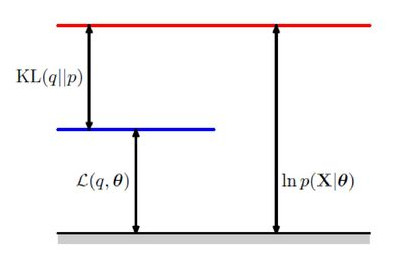
\includegraphics[width=0.4\textwidth]{fig/em-gap.jpg}
\end{figure}


\section*{Solutions to the Exercises}


\solution{M-step-gmm}{For $\bs{\mu}_k$ and $\bs{\Sigma}_k$ re-use the same strategy used for the ML estimators of a multivariate Gaussian distribution in Chapter~\ref{ch:intro}, see Exercise~\ref{ex:ml-estimators-mv-gaussian}. Regarding the $\pi_k$, we need to compute the derivative:
\begin{equation}
 \frac{\partial Q}{\partial \pi_k} = \sum_{n=1}^N \eta_{nk} \frac{1}{\pi_k} - \beta.
\end{equation}
By setting the derivative to zero, we obtain:
\begin{equation}
 \pi_k = \frac{1}{\beta} \sum_{n=1}^N \eta_{nk},
\end{equation}
and we recall that $\sum_k \pi_k = 1$, thus:
\begin{equation}
 1 = \sum_{k=1}^K \pi_k = \frac{1}{\beta} \sum_{k,n=1}^{K,N} \eta_{nk} = \frac{N}{\beta} \Rightarrow \pi_k^* = \frac{1}{N}\sum_{k=1}^N \eta_{nk}. 
\end{equation}

}
